%---------------------------------------------------------------------------------------------------------------------!Draft!-----------------------------------------------------------------------------------------------------------------
\subsection{Espaços conexos por caminhos mas não localmente conexos por caminhos}
\label{localmente-conexo-por-caminhos-ex}
\begin{titlemize}{Lista de dependências}
	\item \hyperref[localmente-conexo-por-caminhos-def]{Espaço localmente conexo por caminhos};\\ %'dependencia1' é o label onde o conceito Dependência 1 aparece (--à arrumar um padrão para referencias e labels--) 
	%\item \hyperref[]{};\\
% quantas dependências forem necessárias.
\end{titlemize}

\begin{ex}[Reta "dobrada"]
	Considere o espaço topológico $\mathbb{R}$ quocientado pela relação de equivalência em que 
    \begin{equation}
        x \sim y \iff x = y \text{ ou } (x = -y \text{ e } x \neq 1)
    \end{equation}
\end{ex}

Com a topologia induzida, o espaço resultante é claramente conexo por caminhos, mas não localmente conexo por caminhos.

\begin{ex}[Círculo Polonês ou de Warsaw]
        Considere o conjunto
    \begin{center}
        $W = \left\{ (x, \sin(\pi / x) : 0 < x < 1 \right\} \cup ( \left\{0\right\} \times [-1, 1] ) \cup \left\{ (x,y) : (x - 1/2)^2 + (y + 15/16)^2 = (17/16)^2 \text{, } y \geqslant 0 \right\}$
    \end{center}
\end{ex}

Esse conjunto é um espaço conexo por caminhos que envolve a \textbf{Curva do Seno do Topólogo}. Nos pontos do segmento $\left\{0\right\} \times [-1, 1]$, W não é localmente conexo por caminhos pelo mesmo motivo que a Curva do Seno do Topólogo original não é conexa por caminhos.

\begin{figure}[t]
    \centering
    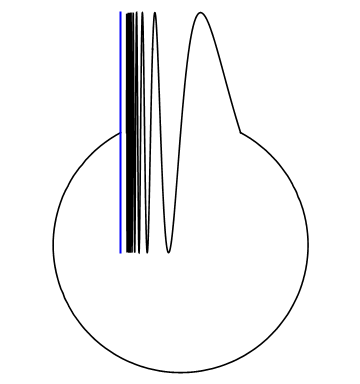
\includegraphics[width=0.4\linewidth]{warsaw.png}
    \caption{Círculo de Warsaw}
    \label{fig:enter-label}
\end{figure}

\begin{titlemize}{Lista de consequências}
	\item \hyperref[levantamento-de-funções-prop]{Levantamento de funções};\\ %'consequencia1' é o label onde o conceito Consequência 1 aparece
	%\item \hyperref[]{}
\end{titlemize}
